\documentclass[conference]{IEEEtran}
\usepackage[T1]{fontenc}
\usepackage{amsmath,amssymb,booktabs,array,tabularx}
\usepackage{xcolor}
\usepackage{graphicx}
\usepackage{tikz}
\usetikzlibrary{arrows.meta,positioning}
\usepackage{cite,url,microtype}
\usepackage[hidelinks]{hyperref}
\hypersetup{pdftitle={Analytical and Learned Atom Ranking for Memory-Enhanced Evolutionary Binary RIS Control}}
\setlength{\emergencystretch}{2em}
\renewcommand{\arraystretch}{1.1}

% results.tex -- populated numbers and decisions of the matched-configuration comparison.
% Primary budget locked on validation: 50 ms. Test evaluations frozen.
\newcommand{\pend}{\textbf{\textcolor{red}{[PENDING]}}}

% ---------------- Per-method metrics at the primary budget (50 ms), test set ----------------
% Rate: mean worst-user SE [bit/s/Hz]; Runtime: p95 complete runtime [ms]; Miss: deadline misses (count/trials);
% Evals: mean evaluations; TttMedian/TttTail: median / p95 time-to-target [ms]; Reached: fraction of runs reaching the target;
% EvalsTarget: mean evaluations used when the target is reached.
\newcommand{\resCplGreedyRate}{15.52535}
\newcommand{\resCplGreedyRuntime}{49.199}
\newcommand{\resCplGreedyMiss}{0/4800}
\newcommand{\resCplGreedyEvals}{24337.0}
\newcommand{\resCplGreedyTttMedian}{0.475}
\newcommand{\resCplGreedyTttTail}{0.674}
\newcommand{\resCplGreedyReached}{0.166}
\newcommand{\resCplGreedyEvalsTarget}{189.5}
\newcommand{\resCplPairRate}{16.23363}
\newcommand{\resCplPairRuntime}{48.972}
\newcommand{\resCplPairMiss}{0/4800}
\newcommand{\resCplPairEvals}{79290.9}
\newcommand{\resCplPairTttMedian}{0.478}
\newcommand{\resCplPairTttTail}{36.487}
\newcommand{\resCplPairReached}{0.201}
\newcommand{\resCplPairEvalsTarget}{7919.5}
\newcommand{\resCplRandomRate}{15.26163}
\newcommand{\resCplRandomRuntime}{49.215}
\newcommand{\resCplRandomMiss}{0/4800}
\newcommand{\resCplRandomEvals}{288.7}
\newcommand{\resCplRandomTttMedian}{0.475}
\newcommand{\resCplRandomTttTail}{0.649}
\newcommand{\resCplRandomReached}{0.163}
\newcommand{\resCplRandomEvalsTarget}{1.0}
\newcommand{\resCplUniformRate}{15.55335}
\newcommand{\resCplUniformRuntime}{9.338}
\newcommand{\resCplUniformMiss}{0/4800}
\newcommand{\resCplUniformEvals}{3394.2}
\newcommand{\resCplUniformTttMedian}{0.476}
\newcommand{\resCplUniformTttTail}{0.664}
\newcommand{\resCplUniformReached}{0.164}
\newcommand{\resCplUniformEvalsTarget}{25.2}
\newcommand{\resCplMemoryRate}{15.62635}
\newcommand{\resCplMemoryRuntime}{10.210}
\newcommand{\resCplMemoryMiss}{0/4800}
\newcommand{\resCplMemoryEvals}{3549.0}
\newcommand{\resCplMemoryTttMedian}{0.475}
\newcommand{\resCplMemoryTttTail}{0.660}
\newcommand{\resCplMemoryReached}{0.164}
\newcommand{\resCplMemoryEvalsTarget}{16.1}
\newcommand{\resCplAnalyticalRate}{15.63728}
\newcommand{\resCplAnalyticalRuntime}{10.214}
\newcommand{\resCplAnalyticalMiss}{0/4800}
\newcommand{\resCplAnalyticalEvals}{3534.0}
\newcommand{\resCplAnalyticalTttMedian}{0.476}
\newcommand{\resCplAnalyticalTttTail}{0.671}
\newcommand{\resCplAnalyticalReached}{0.165}
\newcommand{\resCplAnalyticalEvalsTarget}{48.7}
\newcommand{\resCplAnalyticalNoMemoryRate}{15.55154}
\newcommand{\resCplAnalyticalNoMemoryRuntime}{7.523}
\newcommand{\resCplAnalyticalNoMemoryMiss}{0/4800}
\newcommand{\resCplAnalyticalNoMemoryEvals}{2744.2}
\newcommand{\resCplAnalyticalNoMemoryTttMedian}{0.476}
\newcommand{\resCplAnalyticalNoMemoryTttTail}{0.659}
\newcommand{\resCplAnalyticalNoMemoryReached}{0.163}
\newcommand{\resCplAnalyticalNoMemoryEvalsTarget}{4.3}
\newcommand{\resCplMlpRate}{15.66539}
\newcommand{\resCplMlpRuntime}{11.461}
\newcommand{\resCplMlpMiss}{0/4800}
\newcommand{\resCplMlpEvals}{3609.5}
\newcommand{\resCplMlpTttMedian}{0.476}
\newcommand{\resCplMlpTttTail}{0.675}
\newcommand{\resCplMlpReached}{0.166}
\newcommand{\resCplMlpEvalsTarget}{68.2}
\newcommand{\resCplAttentionRate}{15.65760}
\newcommand{\resCplAttentionRuntime}{12.221}
\newcommand{\resCplAttentionMiss}{0/4800}
\newcommand{\resCplAttentionEvals}{3615.2}
\newcommand{\resCplAttentionTttMedian}{0.475}
\newcommand{\resCplAttentionTttTail}{0.668}
\newcommand{\resCplAttentionReached}{0.166}
\newcommand{\resCplAttentionEvalsTarget}{63.5}
\newcommand{\resCplAttentionNoMemoryRate}{15.55997}
\newcommand{\resCplAttentionNoMemoryRuntime}{9.231}
\newcommand{\resCplAttentionNoMemoryMiss}{0/4800}
\newcommand{\resCplAttentionNoMemoryEvals}{2761.5}
\newcommand{\resCplAttentionNoMemoryTttMedian}{0.476}
\newcommand{\resCplAttentionNoMemoryTttTail}{0.659}
\newcommand{\resCplAttentionNoMemoryReached}{0.164}
\newcommand{\resCplAttentionNoMemoryEvalsTarget}{12.4}
\newcommand{\resCplAttentionNoPhysicsRate}{15.66065}
\newcommand{\resCplAttentionNoPhysicsRuntime}{12.335}
\newcommand{\resCplAttentionNoPhysicsMiss}{0/4800}
\newcommand{\resCplAttentionNoPhysicsEvals}{3583.5}
\newcommand{\resCplAttentionNoPhysicsTttMedian}{0.476}
\newcommand{\resCplAttentionNoPhysicsTttTail}{0.675}
\newcommand{\resCplAttentionNoPhysicsReached}{0.166}
\newcommand{\resCplAttentionNoPhysicsEvalsTarget}{53.3}
\newcommand{\resSpeGreedyRate}{5.44194}
\newcommand{\resSpeGreedyRuntime}{48.841}
\newcommand{\resSpeGreedyMiss}{0/1200}
\newcommand{\resSpeGreedyEvals}{103022.9}
\newcommand{\resSpeGreedyTttMedian}{0.517}
\newcommand{\resSpeGreedyTttTail}{1.020}
\newcommand{\resSpeGreedyReached}{1.000}
\newcommand{\resSpeGreedyEvalsTarget}{694.3}
\newcommand{\resSpePairRate}{5.44247}
\newcommand{\resSpePairRuntime}{48.512}
\newcommand{\resSpePairMiss}{0/1200}
\newcommand{\resSpePairEvals}{196913.8}
\newcommand{\resSpePairTttMedian}{0.516}
\newcommand{\resSpePairTttTail}{1.003}
\newcommand{\resSpePairReached}{1.000}
\newcommand{\resSpePairEvalsTarget}{664.2}
\newcommand{\resSpeRandomRate}{5.42107}
\newcommand{\resSpeRandomRuntime}{48.862}
\newcommand{\resSpeRandomMiss}{0/1200}
\newcommand{\resSpeRandomEvals}{13529.9}
\newcommand{\resSpeRandomTttMedian}{0.297}
\newcommand{\resSpeRandomTttTail}{25.180}
\newcommand{\resSpeRandomReached}{0.496}
\newcommand{\resSpeRandomEvalsTarget}{1018.2}
\newcommand{\resSpeUniformRate}{5.44202}
\newcommand{\resSpeUniformRuntime}{5.755}
\newcommand{\resSpeUniformMiss}{0/1200}
\newcommand{\resSpeUniformEvals}{6921.8}
\newcommand{\resSpeUniformTttMedian}{0.522}
\newcommand{\resSpeUniformTttTail}{0.994}
\newcommand{\resSpeUniformReached}{0.999}
\newcommand{\resSpeUniformEvalsTarget}{601.2}
\newcommand{\resSpeMemoryRate}{5.44232}
\newcommand{\resSpeMemoryRuntime}{7.086}
\newcommand{\resSpeMemoryMiss}{0/1200}
\newcommand{\resSpeMemoryEvals}{8068.9}
\newcommand{\resSpeMemoryTttMedian}{0.526}
\newcommand{\resSpeMemoryTttTail}{1.004}
\newcommand{\resSpeMemoryReached}{1.000}
\newcommand{\resSpeMemoryEvalsTarget}{597.7}
\newcommand{\resSpeAnalyticalRate}{5.44232}
\newcommand{\resSpeAnalyticalRuntime}{6.946}
\newcommand{\resSpeAnalyticalMiss}{0/1200}
\newcommand{\resSpeAnalyticalEvals}{8082.8}
\newcommand{\resSpeAnalyticalTttMedian}{0.516}
\newcommand{\resSpeAnalyticalTttTail}{0.998}
\newcommand{\resSpeAnalyticalReached}{1.000}
\newcommand{\resSpeAnalyticalEvalsTarget}{597.7}
\newcommand{\resSpeAnalyticalNoMemoryRate}{5.44232}
\newcommand{\resSpeAnalyticalNoMemoryRuntime}{7.043}
\newcommand{\resSpeAnalyticalNoMemoryMiss}{0/1200}
\newcommand{\resSpeAnalyticalNoMemoryEvals}{8081.6}
\newcommand{\resSpeAnalyticalNoMemoryTttMedian}{0.510}
\newcommand{\resSpeAnalyticalNoMemoryTttTail}{0.987}
\newcommand{\resSpeAnalyticalNoMemoryReached}{1.000}
\newcommand{\resSpeAnalyticalNoMemoryEvalsTarget}{597.7}
\newcommand{\resSpeMlpRate}{5.44233}
\newcommand{\resSpeMlpRuntime}{7.485}
\newcommand{\resSpeMlpMiss}{0/1200}
\newcommand{\resSpeMlpEvals}{8116.0}
\newcommand{\resSpeMlpTttMedian}{0.513}
\newcommand{\resSpeMlpTttTail}{1.005}
\newcommand{\resSpeMlpReached}{1.000}
\newcommand{\resSpeMlpEvalsTarget}{597.7}
\newcommand{\resSpeAttentionRate}{5.44233}
\newcommand{\resSpeAttentionRuntime}{7.706}
\newcommand{\resSpeAttentionMiss}{0/1200}
\newcommand{\resSpeAttentionEvals}{8112.8}
\newcommand{\resSpeAttentionTttMedian}{0.518}
\newcommand{\resSpeAttentionTttTail}{1.014}
\newcommand{\resSpeAttentionReached}{1.000}
\newcommand{\resSpeAttentionEvalsTarget}{597.7}
\newcommand{\resSpeAttentionNoMemoryRate}{5.44233}
\newcommand{\resSpeAttentionNoMemoryRuntime}{7.678}
\newcommand{\resSpeAttentionNoMemoryMiss}{0/1200}
\newcommand{\resSpeAttentionNoMemoryEvals}{8111.6}
\newcommand{\resSpeAttentionNoMemoryTttMedian}{0.513}
\newcommand{\resSpeAttentionNoMemoryTttTail}{1.007}
\newcommand{\resSpeAttentionNoMemoryReached}{1.000}
\newcommand{\resSpeAttentionNoMemoryEvalsTarget}{597.7}
\newcommand{\resSpeAttentionNoPhysicsRate}{5.44233}
\newcommand{\resSpeAttentionNoPhysicsRuntime}{7.679}
\newcommand{\resSpeAttentionNoPhysicsMiss}{0/1200}
\newcommand{\resSpeAttentionNoPhysicsEvals}{8111.5}
\newcommand{\resSpeAttentionNoPhysicsTttMedian}{0.523}
\newcommand{\resSpeAttentionNoPhysicsTttTail}{1.003}
\newcommand{\resSpeAttentionNoPhysicsReached}{1.000}
\newcommand{\resSpeAttentionNoPhysicsEvalsTarget}{597.7}

% ---------------- Worst-user SE by budget (budgets 1, 5, 10, 50, 100 ms) ----------------
\newcommand{\resCplGreedyRateBOne}{15.26163}
\newcommand{\resCplGreedyRateBFive}{15.30829}
\newcommand{\resCplGreedyRateBTen}{15.35758}
\newcommand{\resCplGreedyRateBFifty}{15.52535}
\newcommand{\resCplGreedyRateBHundred}{15.63880}
\newcommand{\resCplPairRateBOne}{15.26163}
\newcommand{\resCplPairRateBFive}{15.59947}
\newcommand{\resCplPairRateBTen}{15.74698}
\newcommand{\resCplPairRateBFifty}{16.23363}
\newcommand{\resCplPairRateBHundred}{16.50810}
\newcommand{\resCplRandomRateBOne}{15.26163}
\newcommand{\resCplRandomRateBFive}{15.26163}
\newcommand{\resCplRandomRateBTen}{15.26163}
\newcommand{\resCplRandomRateBFifty}{15.26163}
\newcommand{\resCplRandomRateBHundred}{15.26163}
\newcommand{\resCplUniformRateBOne}{15.26877}
\newcommand{\resCplUniformRateBFive}{15.46605}
\newcommand{\resCplUniformRateBTen}{15.54412}
\newcommand{\resCplUniformRateBFifty}{15.55335}
\newcommand{\resCplUniformRateBHundred}{15.55335}
\newcommand{\resCplMemoryRateBOne}{15.26877}
\newcommand{\resCplMemoryRateBFive}{15.57251}
\newcommand{\resCplMemoryRateBTen}{15.61497}
\newcommand{\resCplMemoryRateBFifty}{15.62635}
\newcommand{\resCplMemoryRateBHundred}{15.62635}
\newcommand{\resCplAnalyticalRateBOne}{15.26877}
\newcommand{\resCplAnalyticalRateBFive}{15.55010}
\newcommand{\resCplAnalyticalRateBTen}{15.63175}
\newcommand{\resCplAnalyticalRateBFifty}{15.63728}
\newcommand{\resCplAnalyticalRateBHundred}{15.63728}
\newcommand{\resCplAnalyticalNoMemoryRateBOne}{15.26877}
\newcommand{\resCplAnalyticalNoMemoryRateBFive}{15.51189}
\newcommand{\resCplAnalyticalNoMemoryRateBTen}{15.54885}
\newcommand{\resCplAnalyticalNoMemoryRateBFifty}{15.55154}
\newcommand{\resCplAnalyticalNoMemoryRateBHundred}{15.55154}
\newcommand{\resCplMlpRateBOne}{15.26877}
\newcommand{\resCplMlpRateBFive}{15.58149}
\newcommand{\resCplMlpRateBTen}{15.64995}
\newcommand{\resCplMlpRateBFifty}{15.66539}
\newcommand{\resCplMlpRateBHundred}{15.66539}
\newcommand{\resCplAttentionRateBOne}{15.26877}
\newcommand{\resCplAttentionRateBFive}{15.57085}
\newcommand{\resCplAttentionRateBTen}{15.63630}
\newcommand{\resCplAttentionRateBFifty}{15.65760}
\newcommand{\resCplAttentionRateBHundred}{15.65760}
\newcommand{\resCplAttentionNoMemoryRateBOne}{15.26877}
\newcommand{\resCplAttentionNoMemoryRateBFive}{15.52540}
\newcommand{\resCplAttentionNoMemoryRateBTen}{15.55487}
\newcommand{\resCplAttentionNoMemoryRateBFifty}{15.55997}
\newcommand{\resCplAttentionNoMemoryRateBHundred}{15.55997}
\newcommand{\resCplAttentionNoPhysicsRateBOne}{15.26877}
\newcommand{\resCplAttentionNoPhysicsRateBFive}{15.58080}
\newcommand{\resCplAttentionNoPhysicsRateBTen}{15.64993}
\newcommand{\resCplAttentionNoPhysicsRateBFifty}{15.66065}
\newcommand{\resCplAttentionNoPhysicsRateBHundred}{15.66065}
\newcommand{\resSpeGreedyRateBOne}{5.42781}
\newcommand{\resSpeGreedyRateBFive}{5.44110}
\newcommand{\resSpeGreedyRateBTen}{5.44146}
\newcommand{\resSpeGreedyRateBFifty}{5.44194}
\newcommand{\resSpeGreedyRateBHundred}{5.44206}
\newcommand{\resSpePairRateBOne}{5.42774}
\newcommand{\resSpePairRateBFive}{5.44219}
\newcommand{\resSpePairRateBTen}{5.44236}
\newcommand{\resSpePairRateBFifty}{5.44247}
\newcommand{\resSpePairRateBHundred}{5.44248}
\newcommand{\resSpeRandomRateBOne}{5.41094}
\newcommand{\resSpeRandomRateBFive}{5.41663}
\newcommand{\resSpeRandomRateBTen}{5.41802}
\newcommand{\resSpeRandomRateBFifty}{5.42107}
\newcommand{\resSpeRandomRateBHundred}{5.42226}
\newcommand{\resSpeUniformRateBOne}{5.39947}
\newcommand{\resSpeUniformRateBFive}{5.44194}
\newcommand{\resSpeUniformRateBTen}{5.44201}
\newcommand{\resSpeUniformRateBFifty}{5.44202}
\newcommand{\resSpeUniformRateBHundred}{5.44202}
\newcommand{\resSpeMemoryRateBOne}{5.39947}
\newcommand{\resSpeMemoryRateBFive}{5.44221}
\newcommand{\resSpeMemoryRateBTen}{5.44229}
\newcommand{\resSpeMemoryRateBFifty}{5.44232}
\newcommand{\resSpeMemoryRateBHundred}{5.44232}
\newcommand{\resSpeAnalyticalRateBOne}{5.39947}
\newcommand{\resSpeAnalyticalRateBFive}{5.44221}
\newcommand{\resSpeAnalyticalRateBTen}{5.44230}
\newcommand{\resSpeAnalyticalRateBFifty}{5.44232}
\newcommand{\resSpeAnalyticalRateBHundred}{5.44232}
\newcommand{\resSpeAnalyticalNoMemoryRateBOne}{5.39947}
\newcommand{\resSpeAnalyticalNoMemoryRateBFive}{5.44220}
\newcommand{\resSpeAnalyticalNoMemoryRateBTen}{5.44230}
\newcommand{\resSpeAnalyticalNoMemoryRateBFifty}{5.44232}
\newcommand{\resSpeAnalyticalNoMemoryRateBHundred}{5.44232}
\newcommand{\resSpeMlpRateBOne}{5.39947}
\newcommand{\resSpeMlpRateBFive}{5.44218}
\newcommand{\resSpeMlpRateBTen}{5.44229}
\newcommand{\resSpeMlpRateBFifty}{5.44233}
\newcommand{\resSpeMlpRateBHundred}{5.44233}
\newcommand{\resSpeAttentionRateBOne}{5.39947}
\newcommand{\resSpeAttentionRateBFive}{5.44216}
\newcommand{\resSpeAttentionRateBTen}{5.44227}
\newcommand{\resSpeAttentionRateBFifty}{5.44233}
\newcommand{\resSpeAttentionRateBHundred}{5.44233}
\newcommand{\resSpeAttentionNoMemoryRateBOne}{5.39947}
\newcommand{\resSpeAttentionNoMemoryRateBFive}{5.44216}
\newcommand{\resSpeAttentionNoMemoryRateBTen}{5.44227}
\newcommand{\resSpeAttentionNoMemoryRateBFifty}{5.44233}
\newcommand{\resSpeAttentionNoMemoryRateBHundred}{5.44233}
\newcommand{\resSpeAttentionNoPhysicsRateBOne}{5.39947}
\newcommand{\resSpeAttentionNoPhysicsRateBFive}{5.44216}
\newcommand{\resSpeAttentionNoPhysicsRateBTen}{5.44227}
\newcommand{\resSpeAttentionNoPhysicsRateBFifty}{5.44233}
\newcommand{\resSpeAttentionNoPhysicsRateBHundred}{5.44233}

% ---------------- Paired contrasts at the primary budget: estimate, interval limits, Holm-adjusted p, decision ----------------
% Est/Lo/Hi in bit/s/Hz (first-named method minus second-named); P: Holm-adjusted two-sided bootstrap p; Dec: improved | equivalent | deteriorated | inconclusive | numerically_unresolved.
\newcommand{\resCplCAttMemEst}{0.03125}
\newcommand{\resCplCAttMemLo}{-0.02339}
\newcommand{\resCplCAttMemHi}{0.08487}
\newcommand{\resCplCAttMemP}{0.5089}
\newcommand{\resCplCAttMemDec}{inconclusive}
\newcommand{\resCplCMlpMemEst}{0.03904}
\newcommand{\resCplCMlpMemLo}{-0.01563}
\newcommand{\resCplCMlpMemHi}{0.09345}
\newcommand{\resCplCMlpMemP}{0.3000}
\newcommand{\resCplCMlpMemDec}{inconclusive}
\newcommand{\resCplCAnaMemEst}{0.01093}
\newcommand{\resCplCAnaMemLo}{-0.01112}
\newcommand{\resCplCAnaMemHi}{0.04741}
\newcommand{\resCplCAnaMemP}{0.7823}
\newcommand{\resCplCAnaMemDec}{inconclusive}
\newcommand{\resCplCAttAnaEst}{0.02032}
\newcommand{\resCplCAttAnaLo}{-0.02460}
\newcommand{\resCplCAttAnaHi}{0.06587}
\newcommand{\resCplCAttAnaP}{0.7823}
\newcommand{\resCplCAttAnaDec}{inconclusive}
\newcommand{\resCplCMemPairEst}{-0.60728}
\newcommand{\resCplCMemPairLo}{-0.81612}
\newcommand{\resCplCMemPairHi}{-0.41841}
\newcommand{\resCplCMemPairP}{0.0022}
\newcommand{\resCplCMemPairDec}{deteriorated}
\newcommand{\resCplCAttNoMemEst}{0.09763}
\newcommand{\resCplCAttNoMemLo}{0.02737}
\newcommand{\resCplCAttNoMemHi}{0.18190}
\newcommand{\resCplCAttNoMemP}{0.0054}
\newcommand{\resCplCAttNoMemDec}{numerically\_unresolved}
\newcommand{\resCplCAnaNoMemEst}{0.08574}
\newcommand{\resCplCAnaNoMemLo}{0.02144}
\newcommand{\resCplCAnaNoMemHi}{0.16370}
\newcommand{\resCplCAnaNoMemP}{0.0054}
\newcommand{\resCplCAnaNoMemDec}{numerically\_unresolved}
\newcommand{\resCplCAnaUniEst}{0.08393}
\newcommand{\resCplCAnaUniLo}{0.02041}
\newcommand{\resCplCAnaUniHi}{0.15388}
\newcommand{\resCplCAnaUniP}{0.0056}
\newcommand{\resCplCAnaUniDec}{numerically\_unresolved}
\newcommand{\resSpeCAttMemEst}{0.00001}
\newcommand{\resSpeCAttMemLo}{-0.00000}
\newcommand{\resSpeCAttMemHi}{0.00003}
\newcommand{\resSpeCAttMemP}{0.3878}
\newcommand{\resSpeCAttMemDec}{equivalent}
\newcommand{\resSpeCMlpMemEst}{0.00001}
\newcommand{\resSpeCMlpMemLo}{-0.00000}
\newcommand{\resSpeCMlpMemHi}{0.00003}
\newcommand{\resSpeCMlpMemP}{0.8489}
\newcommand{\resSpeCMlpMemDec}{equivalent}
\newcommand{\resSpeCAnaMemEst}{-0.00000}
\newcommand{\resSpeCAnaMemLo}{-0.00000}
\newcommand{\resSpeCAnaMemHi}{0.00000}
\newcommand{\resSpeCAnaMemP}{0.9967}
\newcommand{\resSpeCAnaMemDec}{equivalent}
\newcommand{\resSpeCAttAnaEst}{0.00001}
\newcommand{\resSpeCAttAnaLo}{0.00000}
\newcommand{\resSpeCAttAnaHi}{0.00003}
\newcommand{\resSpeCAttAnaP}{0.0224}
\newcommand{\resSpeCAttAnaDec}{equivalent}
\newcommand{\resSpeCMemPairEst}{-0.00015}
\newcommand{\resSpeCMemPairLo}{-0.00024}
\newcommand{\resSpeCMemPairHi}{-0.00006}
\newcommand{\resSpeCMemPairP}{0.0022}
\newcommand{\resSpeCMemPairDec}{equivalent}
\newcommand{\resSpeCAttNoMemEst}{0.00000}
\newcommand{\resSpeCAttNoMemLo}{0.00000}
\newcommand{\resSpeCAttNoMemHi}{0.00000}
\newcommand{\resSpeCAttNoMemP}{1.0000}
\newcommand{\resSpeCAttNoMemDec}{equivalent}
\newcommand{\resSpeCAnaNoMemEst}{0.00000}
\newcommand{\resSpeCAnaNoMemLo}{0.00000}
\newcommand{\resSpeCAnaNoMemHi}{0.00000}
\newcommand{\resSpeCAnaNoMemP}{1.0000}
\newcommand{\resSpeCAnaNoMemDec}{equivalent}
\newcommand{\resSpeCAnaUniEst}{0.00029}
\newcommand{\resSpeCAnaUniLo}{0.00013}
\newcommand{\resSpeCAnaUniHi}{0.00052}
\newcommand{\resSpeCAnaUniP}{0.0022}
\newcommand{\resSpeCAnaUniDec}{equivalent}

% ---------------- Sensitivity of the decisions to the shared configuration (validation only) ----------------
\newcommand{\resCplSmallCAttMemDec}{inconclusive}
\newcommand{\resCplSmallCMlpMemDec}{inconclusive}
\newcommand{\resCplSmallCAnaMemDec}{inconclusive}
\newcommand{\resCplSmallCAttAnaDec}{inconclusive}
\newcommand{\resCplSmallCMemPairDec}{deteriorated}
\newcommand{\resCplSmallCAttNoMemDec}{numerically\_unresolved}
\newcommand{\resCplSmallCAnaNoMemDec}{numerically\_unresolved}
\newcommand{\resCplSmallCAnaUniDec}{numerically\_unresolved}
\newcommand{\resCplLargeCAttMemDec}{inconclusive}
\newcommand{\resCplLargeCMlpMemDec}{inconclusive}
\newcommand{\resCplLargeCAnaMemDec}{inconclusive}
\newcommand{\resCplLargeCAttAnaDec}{inconclusive}
\newcommand{\resCplLargeCMemPairDec}{deteriorated}
\newcommand{\resCplLargeCAttNoMemDec}{numerically\_unresolved}
\newcommand{\resCplLargeCAnaNoMemDec}{numerically\_unresolved}
\newcommand{\resCplLargeCAnaUniDec}{numerically\_unresolved}
\newcommand{\resSpeSmallCAttMemDec}{equivalent}
\newcommand{\resSpeSmallCMlpMemDec}{equivalent}
\newcommand{\resSpeSmallCAnaMemDec}{equivalent}
\newcommand{\resSpeSmallCAttAnaDec}{equivalent}
\newcommand{\resSpeSmallCMemPairDec}{equivalent}
\newcommand{\resSpeSmallCAttNoMemDec}{equivalent}
\newcommand{\resSpeSmallCAnaNoMemDec}{equivalent}
\newcommand{\resSpeSmallCAnaUniDec}{equivalent}
\newcommand{\resSpeLargeCAttMemDec}{equivalent}
\newcommand{\resSpeLargeCMlpMemDec}{equivalent}
\newcommand{\resSpeLargeCAnaMemDec}{equivalent}
\newcommand{\resSpeLargeCAttAnaDec}{equivalent}
\newcommand{\resSpeLargeCMemPairDec}{equivalent}
\newcommand{\resSpeLargeCAttNoMemDec}{equivalent}
\newcommand{\resSpeLargeCAnaNoMemDec}{equivalent}
\newcommand{\resSpeLargeCAnaUniDec}{equivalent}

% ---------------- Outcome-dependent sentences ----------------
\newcommand{\resCplSAttMem}{The comparison of \mth{attention\_ga} with \mth{memory\_ga} was inconclusive: the corrected interval is neither above nor within the margin.}
\newcommand{\resCplSMlpMem}{The comparison of \mth{mlp\_ga} with \mth{memory\_ga} was inconclusive: the corrected interval is neither above nor within the margin.}
\newcommand{\resCplSAnaMem}{The comparison of \mth{analytical\_ga} with \mth{memory\_ga} was inconclusive: the corrected interval is neither above nor within the margin.}
\newcommand{\resCplSAttAna}{The comparison of \mth{attention\_ga} with \mth{analytical\_ga} was inconclusive: the corrected interval is neither above nor within the margin.}
\newcommand{\resCplSMemPair}{The comparison of \mth{memory\_ga} with \mth{pair} showed deterioration: the corrected interval lies entirely below the practical margin.}
\newcommand{\resCplSAttNoMem}{\mth{attention\_ga} exceeded \mth{attention\_no\_memory\_ga} statistically above the practical margin, but the contrast remains numerically unresolved pending the fine-mesh audit.}
\newcommand{\resCplSAnaNoMem}{\mth{analytical\_ga} exceeded \mth{analytical\_no\_memory\_ga} statistically above the practical margin, but the contrast remains numerically unresolved pending the fine-mesh audit.}
\newcommand{\resCplSAnaUni}{\mth{analytical\_ga} exceeded \mth{uniform\_ga} statistically above the practical margin, but the contrast remains numerically unresolved pending the fine-mesh audit.}
\newcommand{\resSpeSAttMem}{\mth{attention\_ga} and \mth{memory\_ga} were equivalent within the practical margin: the corrected interval lies entirely within it.}
\newcommand{\resSpeSMlpMem}{\mth{mlp\_ga} and \mth{memory\_ga} were equivalent within the practical margin: the corrected interval lies entirely within it.}
\newcommand{\resSpeSAnaMem}{\mth{analytical\_ga} and \mth{memory\_ga} were equivalent within the practical margin: the corrected interval lies entirely within it.}
\newcommand{\resSpeSAttAna}{\mth{attention\_ga} and \mth{analytical\_ga} were equivalent within the practical margin: the corrected interval lies entirely within it.}
\newcommand{\resSpeSMemPair}{\mth{memory\_ga} and \mth{pair} were equivalent within the practical margin: the corrected interval lies entirely within it.}
\newcommand{\resSpeSAttNoMem}{\mth{attention\_ga} and \mth{attention\_no\_memory\_ga} were equivalent within the practical margin: the corrected interval lies entirely within it.}
\newcommand{\resSpeSAnaNoMem}{\mth{analytical\_ga} and \mth{analytical\_no\_memory\_ga} were equivalent within the practical margin: the corrected interval lies entirely within it.}
\newcommand{\resSpeSAnaUni}{\mth{analytical\_ga} and \mth{uniform\_ga} were equivalent within the practical margin: the corrected interval lies entirely within it.}

% Experiment-level and paper-level sentences.
\newcommand{\resCplDiscussion}{In the coupled wire experiment, \mth{pair} local search substantially outperformed all GA variants by over $0.60$~bit/s/Hz at the 50~ms primary budget, with zero deadline misses. Comparisons between neural guidance and analytical or memory baselines were inconclusive, while memory ablation contrasts remained numerically unresolved pending fine-mesh verification.}
\newcommand{\resSpeDiscussion}{In the independent-cell experiment, all 11 contrasts were equivalent within the $\pm 0.015$~bit/s/Hz practical margin at the 50~ms primary budget, with zero deadline misses. All methods reached the target threshold within approximately 1~ms.}
\newcommand{\resCrossDiscussion}{Across both experiments, learned neural ranking did not demonstrate an advantage over analytical ranking or exact local search within the practical margin. The two experiments differ in surface physics, geometry and scene, so agreement or disagreement between them is not an effect of mutual coupling.}
\newcommand{\resAbstractOutcome}{On held-out test trajectories at the locked 50~ms primary budget, all specular contrasts were equivalent within the practical margin; in coupled wire, exact pair search outperformed all GA variants, neural guidance was inconclusive against analytical and memory baselines, and memory ablations remained numerically unresolved pending fine-mesh auditing.}
\newcommand{\resConclusionOutcome}{At the locked 50~ms primary budget on held-out test trajectories, all contrasts in the independent-cell experiment were equivalent within the $\pm 0.015$~bit/s/Hz margin. In the coupled-wire experiment, exact pair search dominated the heuristic GA controllers by over $0.60$~bit/s/Hz, neural ranking showed no conclusive gain over analytical ranking, and memory ablations require fine-mesh resolution.}
\newcommand{\resSensitivitySummary}{Under both the small and large shared configurations on validation data, the contrast decisions were identical to the primary configuration: all specular contrasts remained equivalent, neural-versus-analytical coupled contrasts remained inconclusive, \mth{memory\_ga}$-$\mth{pair} remained deteriorated, and memory ablations remained numerically unresolved.}
\newcommand{\resDeadlineSummary}{At the 50~ms primary budget, zero deadline misses occurred across all 1{,}200 runs in Experiment~S and all 4{,}800 runs in Experiment~C. At the 10~ms budget, Experiment~S had zero misses while Experiment~C experienced 72 misses (principally in neural methods: 19 for \mth{attention\_ga}, 14 for \mth{mlp\_ga}), justifying the locked 50~ms primary budget.}
\newcommand{\resHardwareCPU}{AMD Ryzen 5 5600 6-Core Processor (pinned Core~3, base 3.5~GHz)}
\newcommand{\resSpeFrameReference}{5.44249}
\newcommand{\resCplFrameReference}{17.70736}
% placeholder macros for every matched-comparison number or decision

\newcommand{\bvec}{\mathbf b}
\newcommand{\mth}[1]{\begingroup\renewcommand{\_}{\textunderscore\allowbreak}\texttt{#1}\endgroup}
\newcommand{\margin}{\delta}
\DeclareMathOperator*{\argmax}{arg\,max}
\newcommand{\TODO}[1]{\textbf{\textcolor{red}{[TODO: #1]}}}

\begin{document}

% TODO(authors): confirm author names, affiliations and e-mail addresses before submission. Do not guess.
\title{Analytical and Learned Atom Ranking for Memory-Enhanced Evolutionary Binary RIS Control: A Matched-Budget Simulation Study}
\author{\IEEEauthorblockN{Author names to be confirmed}
\IEEEauthorblockA{Affiliation and contact details to be confirmed}}
\maketitle

\begin{abstract}
Binary reconfigurable intelligent surfaces (RISs) can be controlled by evolutionary search that reuses remembered configurations. Whether a learned per-element ranking of candidate edits helps beyond an analytical ranking, and whether memory helps at all, is easily confounded by method-specific search limits and by neural inference time. This paper specifies and reports a matched-configuration comparison in which eight search variants share one step sequence, one set of limits and one wall-clock deadline, and differ only in the ranking signal and in whether memory is enabled. They are compared with greedy, exact pair and random search on two simulated 64-element worst-user spectral-efficiency problems: an independent-cell surface in a ray-traced urban scene and a 3D thin-wire surface with full mutual coupling. Each problem uses 30 held-out receiver trajectories, ten optimizer seeds and CPU budgets of 1 to 100 ms that include feature extraction and inference. Decisions use paired trajectory bootstrap intervals, Holm correction and a predeclared practical margin of 0.015~bit/s/Hz. \resAbstractOutcome{} The study is simulation-only, assumes complete network observation, and tests held-out trajectories in the same scene, not a held-out environment.
\end{abstract}

\begin{IEEEkeywords}
Reconfigurable intelligent surface, evolutionary memory, learned mutation, attention, mutual coupling, matched comparison.
\end{IEEEkeywords}

\section{Introduction}
A reconfigurable intelligent surface (RIS) steers radio propagation by switching many small elements among discrete electrical states. A binary surface with $N=64$ elements has $2^{64}$ configurations, but this count alone does not show that evolutionary or neural search is needed: the ideal single-user binary problem admits an efficient optimal solution~\cite{zhang}, discrete analytical optimization is a strong competitor for coupled models~\cite{hammami}, and low-rank updates make exact evaluation of single and paired bit edits inexpensive~\cite{prodhomme}. A learned controller must therefore be compared with analytical search that receives the same computational shortcuts.

Memory-enhanced evolutionary control reuses previously good configurations when the channel changes~\cite{zardi}, learned genetic operators have been proposed for generic black-box problems~\cite{lange}, and neural RIS optimizers with domain knowledge exist~\cite{risnet}. A natural question follows: when the search is otherwise identical, does ranking the candidate elements by a learned score, by an analytical score, by the variability of remembered patterns, or at random, change the worst-user rate achieved before a deadline that includes the cost of inference?

Earlier internal development pilots on the two problems studied here used search limits that were set separately for each method. Differences between methods in those pilots cannot be attributed to the ranking signal, because the limits differed as well. This paper therefore freezes a single shared search configuration before any test frame is generated and compares methods on trajectories never used for method design. The registered specification is \texttt{configs/experiments/matched\_v1.json} of the accompanying repository.

\subsection*{Contributions}
% NOVELTY-REVIEW: the statements below describe what is done. They make no claim of novelty and are to be revised
% against docs/novelty-analysis.md when that analysis is available. Do not claim attention, memory, or physics
% conditioning as novel by themselves.
The paper does the following.
\begin{enumerate}
\item % NOVELTY-REVIEW
It specifies a matched-configuration protocol for binary RIS search in which all genetic-algorithm (GA) variants run the same step sequence and limits, and neural overhead is paid from the same deadline (Sections~\ref{sec:controllers} and~\ref{sec:protocol}).
\item % NOVELTY-REVIEW
It defines two simulated worst-user problems with a common objective and a fixed regularized zero-forcing precoder: an independent-cell ray-traced surface and a fully coupled 3D wire surface (Section~\ref{sec:system}).
\item % NOVELTY-REVIEW
It compares eight GA variants, which differ only in ranking signal and memory, with greedy, pair and random search, using complete-runtime and evaluation-count metrics (Section~\ref{sec:protocol}).
\item % NOVELTY-REVIEW
It fixes the statistical decision rule, including a practical margin, before the test benchmark is run, and reports the outcome using placeholders until the frozen benchmark exists (Sections~\ref{sec:results} and~\ref{sec:discussion}).
\end{enumerate}

\section{Related Work}\label{sec:related}
\subsection{Learning-based RIS configuration}
Neural networks have been used to predict discrete RIS states directly. A deep quantization network predicts transmit beamforming and discrete RIS phases for multiuser MISO with imperfect channel information~\cite{xu}. Convolutional networks map a target direction to the binary cell states of arrays of $10\times10$ to $20\times20$ elements and have been implemented on edge processors and FPGAs~\cite{martin,padial}. Urbinati et al.\ score candidate codebook configurations with MLPs and measure inference latency and memory on microcontrollers~\cite{urbinati}. These controllers emit a configuration in one pass and operate under objectives that differ from ours; we neither reproduce them nor claim any hardware result.

\subsection{Evolutionary memory and learned operators}
Zardi et al.\ combine memory-enhanced evolutionary search with electromagnetically characterized meta-atom responses to maximize worst-user throughput under fixed base-station beamforming~\cite{zardi}. Lange et al.\ learn attention-based selection and mutation-rate operators for generic optimization tasks by meta-black-box optimization~\cite{lange}. Liu et al.\ combine a physics-informed surrogate with binary multiobjective optimization for programmable metasurfaces, validated by full-wave simulation~\cite{liuphys}. Our \mth{memory\_ga} variant is an adaptation inspired by~\cite{zardi}, not a reproduction (Section~\ref{sec:controllers}).

\subsection{Mutual coupling and multiport models}
Multiport network theory gives equivalent impedance, admittance and scattering descriptions of RISs that include mutual coupling and mismatch~\cite{nerini}, with explicit electromagnetic and power constraints~\cite{nossek} and full-wave method-of-moments validation of S-parameter designs~\cite{abrardo}. Qian and Di Renzo optimize unit-cell and coupling-aware RISs through mutual impedances~\cite{qian}. Zheng et al.\ train and validate a scattering-matrix model of a fabricated 1-bit RIS against full-wave and measured S-parameters~\cite{zheng}. Peng et al.\ propose a domain-informed neural architecture with mutual coupling and partial channel information~\cite{risnet}. Nerini et al.\ show for beyond-diagonal surfaces that coupling can help or hurt depending on how the surface is optimized~\cite{nerini2}. PhysFad provides coupled-dipole end-to-end channel models~\cite{physfad}. Efficient low-rank updates of interaction matrices~\cite{prodhomme} and statistical multiport models with efficient discrete optimization, including coordinate descent~\cite{hammami}, are the basis for the strong analytical baselines used here.

\subsection{Hardware, measurement and simulation resources}
The surface responses of the independent-cell experiment are taken from plots of the open-source 5~GHz RIS design~\cite{heinrichs}. Public RIS measurement collections at 5~GHz and sub-6~GHz~\cite{tewes,piana,rossanese} and simulation platforms~\cite{qris} are relevant for future external validation but are not used here. Propagation paths are exported through DeepMIMO tooling~\cite{deepmimo}. Temporal channel prediction~\cite{liu22} is outside the scope of this comparison, which concerns spatial control with current network observations only.

\section{System Model and Objective}\label{sec:system}
\subsection{Common objective}
Let $\bvec\in\{0,1\}^N$ be the RIS configuration with $N=64$ binary elements (atoms), $M=4$ base-station (BS) antennas and $K=2$ single-antenna users. For each frame, a precoder $\mathbf W\in\mathbb C^{M\times K}$ is computed once and held fixed for all candidate configurations and all methods. It is the regularized zero-forcing (RZF) precoder of the effective channel with all elements OFF, scaled to total power $\|\mathbf W\|_F^2=P_{\mathrm T}=0.1$~W. Let $\mathbf U(\bvec)\in\mathbb C^{K\times K}$ be the effective stream matrix, whose entry $U_{kj}$ is the received amplitude of stream $j$ at user $k$. The rate of user $k$ and the objective are
\begin{align}
R_k(\bvec)&=\log_2\!\left(1+\frac{|U_{kk}(\bvec)|^2}{\sum_{j\neq k}|U_{kj}(\bvec)|^2+\sigma^2}\right),\label{eq:rate}\\
F(\bvec)&=\min_{1\le k\le K}R_k(\bvec),\qquad \bvec^\star=\argmax_{\bvec}F(\bvec),\label{eq:obj}
\end{align}
with $\sigma^2=k_{\mathrm B}T B\,10^{\mathrm{NF}/10}$, $T=290$~K, $B=1$~MHz and a noise figure $\mathrm{NF}=7$~dB. The reported quantity is the worst-user spectral efficiency (SE) in bit/s/Hz, recomputed with the full evaluator for the configuration each method returns. Using the all-OFF effective channel for the precoder avoids assigning no stream to a user whose direct path is blocked. Channel information is complete and exact for every method: the matched comparison does not test imperfect or stale observations, and the cost of acquiring a complete network description is not modeled.

The two experiments below differ in how $\mathbf U(\bvec)$ is produced. They also differ in geometry, scene and surface hardware model. They are therefore \emph{separate experiments}, not a coupling ablation: absolute rates from one cannot be compared with the other, and neither experiment is a before/after condition of the other.

\subsection{Experiment S: independent-cell surface in a ray-traced scene}
Experiment S uses an $8\times8$ array of independent scalar cells in a Munich urban scene, traced at a nominal carrier of 5.53~GHz using line-of-sight and specular paths. Let $\mathbf D\in\mathbb C^{K\times M}$ be the direct BS-to-user channel, $\mathbf G\in\mathbb C^{N\times M}$ the BS-to-cell channel and $\mathbf H\in\mathbb C^{K\times N}$ the cell-to-user channel. With cell response $\Gamma_n(b_n)$,
\begin{equation}
U_{kj}(\bvec)=(\mathbf D\mathbf W)_{kj}+\frac{4\pi A}{\lambda^2}\sum_{n=1}^{N}H_{kn}\,\Gamma_n(b_n)\,(\mathbf G\mathbf W)_{nj},\label{eq:specular}
\end{equation}
where $A=20\times13$~mm$^2$ is the cell area and $\lambda$ the wavelength; each propagation loss and the cell response enter once. The two state responses are digitized from published plots of a uniformly switched $16\times16$ open-source panel at normal incidence~\cite{heinrichs} and are applied to a smaller mixed-state array and oblique illumination; at 5.53~GHz they are approximately $-5.1$~dB at $-170^\circ$ and $-1.8$~dB at $+9^\circ$. The model contains no mutual coupling, element-specific calibration, cross-polarization or switching-circuit effects. Diffraction was excluded because it did not converge sufficiently in the checked settings; this is a limitation of the scene model, not evidence that diffraction is negligible.

Figure~\ref{fig:munich} locates the BS, virtual RIS probes and receiver tracks in the Sionna Munich scene exported through DeepMIMO~\cite{deepmimo}; it depicts only the independent-cell scene.

\begin{figure*}[t]
\centering
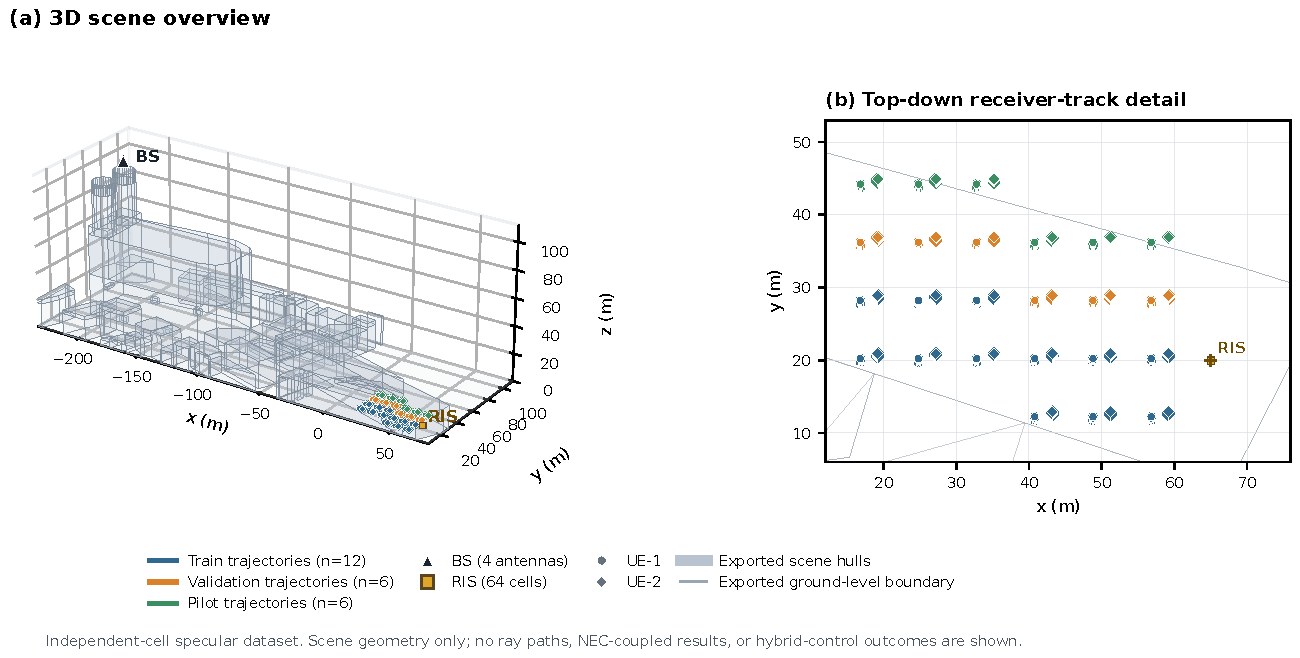
\includegraphics[width=\textwidth]{figures/munich_scene.pdf}
\caption{Scene geometry for the independent-cell specular evaluation: the Sionna Munich scene exported through DeepMIMO as hull geometry (3D overview and top-down receiver-track region). The original four-antenna BS, 64 virtual RIS-cell probes and 24 receiver trajectories (train, validation and pilot) are shown. The exported hulls are a visualization, not an assertion of exact ray-tracing-mesh correspondence; the top-down projection does not establish indoor/outdoor status. This is separate from the NEC-2 coupled-wire model; no hybrid results, human movement or blockage, or V2 outcomes are depicted.}
\label{fig:munich}
\end{figure*}

\subsection{Experiment C: coupled 3D wire surface}
Experiment C replaces the cell model by a free-space, perfectly conducting thin-wire surface solved by the method of moments (NEC-2). Sixty-four vertically polarized wires, each 24~mm long with 50~$\mu$m radius, are placed with horizontal and vertical pitches of 28~mm and 30~mm. Four BS antennas and two user antennas bring the model to 70 ports at 5.53~GHz. Each RIS port is loaded with one of two impedances, $1-j10.799~\Omega$ (state~0) or $1+j129.201~\Omega$ (state~1). There is no substrate, ground plane, switch model, conductor loss, city geometry or human blockage.

Unit-voltage excitations give the full impedance matrix $\mathbf Z$. Order the ports as RIS elements, BS antennas, user antennas and let the external (BS and user) ports be terminated by $Z_0=50~\Omega$ references. The exact Schur reduction onto the RIS ports yields matrices $\mathbf A$, $\mathbf C$, $\mathbf F$ and $\mathbf D_0$ that do not depend on $\bvec$ (the formulas are given in the repository), such that, with RIS loads $\ell_n(b_n)$,
\begin{equation}
\mathbf H(\bvec)=\mathbf D_0+\mathbf C\,\bigl(\mathbf A+\operatorname{diag}\boldsymbol\ell(\bvec)\bigr)^{-1}\mathbf F,\qquad \mathbf U(\bvec)=\mathbf H(\bvec)\mathbf W,\label{eq:coupled}
\end{equation}
mapping incident BS power waves to received user power waves; the factor $2Z_0=100~\Omega$ is absorbed into $\mathbf C$ and $\mathbf D_0$. The power $P_{\mathrm T}$ is the incident, not the radiated, power, because source mismatch and mutual coupling are retained.

A separate development illustration shows the NEC-2 free-space thin-wire geometry used in Experiment C, distinct from the Munich scene.

\begin{figure*}[t]
\centering
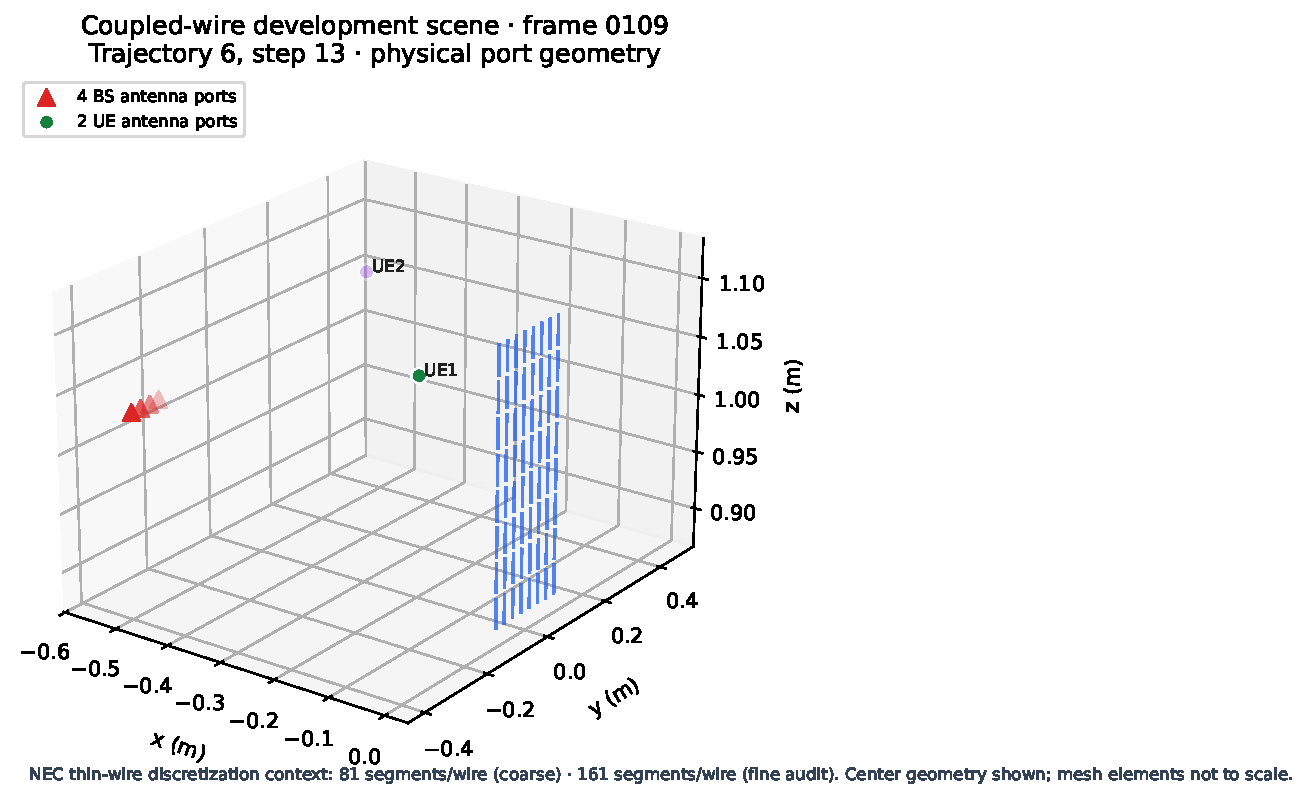
\includegraphics[width=0.82\textwidth]{figures/coupled_wire_geometry.pdf}
\caption{Actual NEC-2 development frame 0109 (trajectory 6, step 13): 64 vertical RIS wires, four BS ports and two UE ports at their port-center coordinates in meters. This ideal PEC free-space wire model has no PCB, city geometry or human blockers. The frame is illustrative only; it reports no controller outcome or mesh-convergence result.}
\label{fig:coupledwiregeom}
\end{figure*}

\subsection{Exact incremental evaluation}
Both evaluators score single and paired bit flips without recomputing $\mathbf U$ from scratch, and every method uses these updates. In Experiment S, flipping element $n$ adds a rank-one term, $\mathbf U(\bvec\oplus\mathbf e_n)=\mathbf U(\bvec)+\mathbf\Delta_n$ with $\mathbf\Delta_n=\tfrac{4\pi A}{\lambda^2}\bigl(\Gamma_n(1-b_n)-\Gamma_n(b_n)\bigr)\mathbf h_n(\mathbf G\mathbf W)_{n,:}$, and two flips add two such terms. In Experiment C, with $\mathbf T=(\mathbf A+\operatorname{diag}\boldsymbol\ell)^{-1}$ cached for the current state and $\epsilon_n=\ell_n(1-b_n)-\ell_n(b_n)$, the Sherman--Morrison identity gives
\begin{equation}
\bigl(\mathbf A+\operatorname{diag}\boldsymbol\ell+\epsilon_n\mathbf e_n\mathbf e_n^{\!\top}\bigr)^{-1}=\mathbf T-\frac{\mathbf T\mathbf e_n\mathbf e_n^{\!\top}\mathbf T}{1/\epsilon_n+T_{nn}},\label{eq:sm}
\end{equation}
and a rank-two Woodbury update handles pairs. Since the evaluation of $F$ uses the same updates for analytical and learned controllers, differences in returned rate are not caused by cheaper physics for one method. Tests in the repository compare these updates with full solves.

\subsection{Numerical evidence for the coupled model}
In the development data of Experiment C, doubling the mesh from 81 to 161 segments per wire changed the complex channel by at most 0.740\% and the worst-user SE by at most 0.01503~bit/s/Hz over 103 reference binary patterns; direct loaded NEC solutions agreed with the network-reduced currents to $7.41\times10^{-14}$ relative norm. This is numerical convergence, not accuracy against a fabricated device. The largest SE change under mesh doubling is the basis of the practical margin used in Section~\ref{sec:protocol}. A separate audit in the development pilot found larger SE changes for returned actions on one frame (Section~\ref{sec:discussion}).

\section{Controllers and Shared Configuration}\label{sec:controllers}
\subsection{Shared step sequence}
All GA variants execute the same step sequence with the same limits (Fig.~\ref{fig:steps}). Starting from the all-OFF configuration, the search (i) climbs by best single flips and by exact pair moves restricted to a ranked subset of atoms, (ii) escapes an all-OFF trap with a random immigrant when the budget permits, (iii) rescores remembered configurations on the current frame and climbs from them, (iv) jumps to nearby basins formed by flipping the highest-ranked atoms and climbs again, and (v) repeats the jump from secondary rank positions. Experiment S additionally evaluates the all-ON basin and a crossover between basins. A candidate returned after the deadline is discarded. \TODO{verify this paragraph against the frozen code snapshot and its hash before submission}

\begin{figure}[t]
\centering
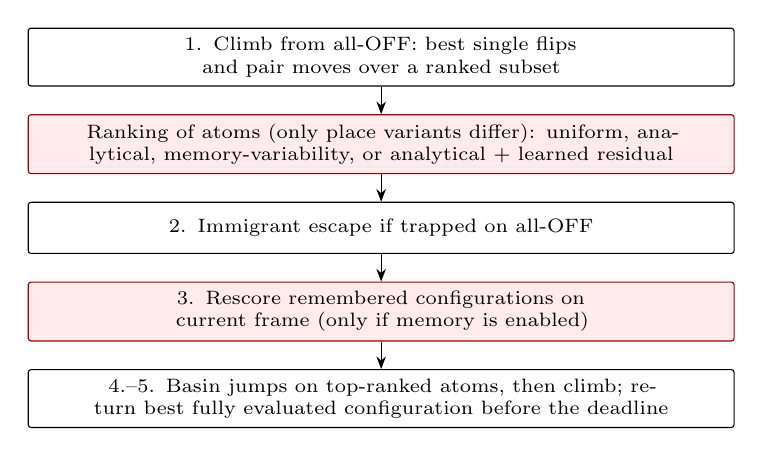
\begin{tikzpicture}[node distance=3.5mm,
  box/.style={draw,rounded corners=1pt,align=center,font=\scriptsize,minimum height=6.5mm,text width=0.72\columnwidth},
  var/.style={box,fill=red!8,draw=red!60!black}]
 \node[box] (a) {1. Climb from all-OFF: best single flips and pair moves over a ranked subset};
 \node[var,below=of a] (b) {Ranking of atoms (only place variants differ): uniform, analytical, memory-variability, or analytical + learned residual};
 \node[box,below=of b] (c) {2. Immigrant escape if trapped on all-OFF};
 \node[var,below=of c] (d) {3. Rescore remembered configurations on current frame (only if memory is enabled)};
 \node[box,below=of d] (e) {4.--5. Basin jumps on top-ranked atoms, then climb; return best fully evaluated configuration before the deadline};
 \draw[-{Stealth[length=1.6mm]}] (a)--(b); \draw[-{Stealth[length=1.6mm]}] (b)--(c);
 \draw[-{Stealth[length=1.6mm]}] (c)--(d); \draw[-{Stealth[length=1.6mm]}] (d)--(e);
\end{tikzpicture}
\caption{Shared search sequence. Shaded blocks are the only two places where the variants differ. Limits (Table~\ref{tab:config}) are identical for all variants.}
\label{fig:steps}
\end{figure}

\subsection{Ranking signals}
At the current state, let $g_n$ be the exact objective change of flipping atom $n$ alone, and $\tilde g_n=g_n/\max(\operatorname{std}(\mathbf g),\varepsilon)$ its normalization. A variant's ranking score $s_n$ is
\begin{equation}
s_n=\begin{cases}
u_n\sim\mathcal U(0,1) & \text{uniform},\\
\tilde g_n & \text{analytical},\\
\tilde g_n+0.1\,\sigma_n & \text{memory},\\
\tilde g_n+w\,\tilde r_n & \text{learned},
\end{cases}\label{eq:rank}
\end{equation}
where $\sigma_n$ is the per-bit standard deviation of the remembered patterns, $\tilde r_n$ is the standardized learned residual and $w$ is a fixed residual weight (Table~\ref{tab:config}). The \emph{memory} score is our adaptation of the memory-enhanced search of Zardi et al.~\cite{zardi}: it keeps their idea of reusing remembered patterns, but it is not a reproduction. The adaptation is evaluated on our objective and information model, not on theirs. In particular, it uses 64 atoms with two states, two users and a different physical model, whereas Zardi et al.\ report 2025 atoms at 3 bits, 900 BS antennas, three users, zero-forcing precoding at 3.5~GHz, with results shown only as plots and without latency. Numerical results here cannot be compared with theirs.

\subsection{Variants}
Table~\ref{tab:variants} lists the eight GA variants and the three baselines. The GA variants differ only in the ranking signal and in whether memory is supplied. \mth{uniform\_ga} is a lesion control for whether ranking matters. \mth{attention\_no\_physics\_ga} removes the explicit physics features but keeps the analytical flip gains, so it is not a physics-free controller.

\begin{table}[t]
\caption{Compared methods. All GA variants share the step sequence and limits.}\label{tab:variants}
\centering\scriptsize
\begin{tabular}{@{}p{0.38\columnwidth}p{0.38\columnwidth}p{0.09\columnwidth}@{}}
\toprule
Method & Ranking signal & Memory\\
\midrule
\mth{uniform\_ga} & uniform random & on\\
\mth{memory\_ga} & $\tilde g+0.1\sigma$ (no network) & on\\
\mth{analytical\_ga} & $\tilde g$ & on\\
\mth{analytical\_no\_memory\_ga} & $\tilde g$ & off\\
\mth{mlp\_ga} & $\tilde g$ + MLP residual & on\\
\mth{attention\_ga} & $\tilde g$ + attention residual & on\\
\mth{attention\_no\_memory\_ga} & as \mth{attention\_ga} & off\\
\mth{attention\_no\_physics\_ga} & as \mth{attention\_ga}, physics features removed, $\tilde g$ kept & on\\
\midrule
\mth{greedy} & best single flip, random restarts & n/a\\
\mth{pair} & best single flip, else best exact pair, random restarts & n/a\\
\mth{random} & random configurations & n/a\\
\bottomrule
\end{tabular}
\end{table}

\subsection{Learned models and training}
Both learned variants return $\tilde g_n$ plus a learned per-atom residual. The \emph{attention} policy embeds per-atom features to width 32, applies two Transformer-encoder layers with four heads and feed-forward width 64 over the atoms, and outputs one scalar per atom. The \emph{MLP} policy sees each atom's features concatenated with the mean over atoms and a context vector weighted by the first-flip marker, and uses two hidden layers of width 96. In Experiment C the per-atom features are the current bit, normalized grid position, exact flip gain, real and imaginary parts of the diagonal of the cached inverse, a summed off-diagonal interaction magnitude, user-side and source-side coupling terms, and a first-flip marker. The attention model has no explicit edge bias between atoms. In the development pilots the parameter counts were 14{,}113 (MLP) and 17{,}665 (attention) for Experiment C and 18{,}145 (MLP) and 18{,}113 (attention) for Experiment S.

Models are supervised with the softmax over completed single- and pair-flip gains of training parents, including pairs whose first flip alone is harmful, and trained with AdamW (learning rate $3\times10^{-4}$, weight decay $10^{-3}$, gradient clipping at 1) for 25 epochs, keeping the checkpoint with the lowest validation loss. For the matched comparison, a fresh checkpoint is trained for every seed from the training and validation splits only; epochs and architectures are unchanged from the development pilots. Training cost is not charged to the online budget, whereas feature extraction and inference are.

\subsection{Shared configuration and its sensitivity}
Table~\ref{tab:config} lists the limits shared by all GA variants. The medium setting equals the values previously assigned to \mth{analytical\_ga} and was fixed without consulting any matched result; small and large settings are run on validation data only, to show whether conclusions depend on the configuration, and are never used to change the primary setting. Neural overhead is paid from the same deadline, so a learned variant that spends time on inference has correspondingly less time for search.

\begin{table}[t]
\caption{Shared search limits (registered). Experiment C: $K$ ranked atoms for subset pair moves, $K_{\mathrm{hop}}$ for basin climbs. Experiment S: $P_0,P_1$ anchor counts, $n_{\mathrm{starts}}$ extra starts, $\max_{\mathrm{pol}}$ policy passes, $t_{\mathrm{cap}}$ cap fractions of the budget (ms limit applies to budgets up to 12~ms). All variants: hop atoms $\{0,1\}$ of the ranking; secondary hops on; basin crossover on (S); residual weight 0.12 (C), 0.15 (S); memory bias weight 0.1.}\label{tab:config}
\centering\footnotesize
\begin{tabular}{@{}lccc@{}}
\toprule
 & Small & \textbf{Medium} & Large\\
\midrule
C: $K$ / $K_{\mathrm{hop}}$ & 18 / 14 & \textbf{20 / 16} & 28 / 20\\
S: $P_0$ / $P_1$ & 4 / 3 & \textbf{5 / 4} & 6 / 5\\
S: $n_{\mathrm{starts}}$ / $\max_{\mathrm{pol}}$ & 0 / 1 & \textbf{1 / 2} & 4 / 4\\
S: $t_{\mathrm{cap}}$ fraction, short / long & 0.45 / 0.50 & \textbf{0.52 / 0.58} & 0.65 / 0.72\\
S: $t_{\mathrm{cap}}$ limit, short (ms) & 3.2 & \textbf{3.8} & 5.4\\
\bottomrule
\end{tabular}
\end{table}

\subsection{Baselines}
\mth{greedy} flips the best single atom until none improves and then restarts from a random configuration; \mth{pair} additionally evaluates all exact pair moves when no single flip improves; \mth{random} scores random configurations. They use the same exact incremental evaluation and the same counting rule as the GA variants, do not follow the GA step sequence, and have no per-method limits to tune, so they are outside the shared GA configuration. \TODO{state whether the registered benchmark gives the baselines remembered patterns in each experiment}

\section{Experimental Protocol}\label{sec:protocol}
\subsection{Data and splits}
Table~\ref{tab:data} summarizes the data. Splits are made over whole trajectories before any label or test frame is generated. The development pilot trajectories of the earlier experiments informed method design; they are excluded from training and validation in the matched comparison and are never reported as the test result. The test set is generated once, after the method design is frozen, from a registered random seed (20261106). Test receiver positions and velocities of Experiment C are drawn continuously and uniformly over the bounding box of the existing user start positions and velocities, with the same physics, surface and 81 segments per wire. Test trajectories of Experiment S are new receiver trajectories in the same scene with the same ray-tracing parameters. Held-out trajectories in the same scene and surface are not a held-out environment: they do not test transfer to another surface, scene or hardware.

\begin{table}[t]
\caption{Data of the matched comparison.}\label{tab:data}
\centering\scriptsize
\begin{tabular}{@{}p{0.22\columnwidth}p{0.33\columnwidth}p{0.33\columnwidth}@{}}
\toprule
 & Experiment C (coupled wire) & Experiment S (independent cell)\\
\midrule
Surface & 64 wires, NEC-2 & $8\times8$ scalar cells\\
Scene & free space, moving users & Munich urban scene\\
Users / BS antennas & 2 / 4 & 2 / 4\\
Train and validation data & 6 + 3 trajectories (\texttt{coupled\_wire\_v1}) & 12 + 6 trajectories (\texttt{munich\_specular\_v3})\\
Test trajectories & 30 & 30\\
Frames per trajectory & 16 & 4\\
Test frames & 480 & 120\\
\bottomrule
\end{tabular}
\end{table}

\subsection{Seeds, budgets and timing}
Ten optimizer seeds ($7, 19, 43, 3, 11, 23, 31, 59, 67, 83$) are used for every method and frame. CPU budgets are 1, 5, 10, 50 and 100~ms; 10~ms was the preferred budget, and 50~ms is the locked primary budget selected on validation due to deadline misses at 10~ms. All timing is measured on one lab node on one pinned CPU core, single-threaded, with no concurrent job of ours (CPU: \resHardwareCPU). Methods run sequentially. The budget for a method begins when the frame is handed to it and covers preparation, feature extraction, neural inference, memory handling and candidate evaluation. One-time model loading, channel acquisition, electromagnetic simulation and the later scoring of the returned action are excluded. \TODO{confirm the exclusion list against the final benchmark scripts} Deadlines are soft: candidates completed after the deadline cannot become the returned action, and the actual overrun is recorded.

\subsection{Freeze order}
The order is fixed: (1) train; (2) run the validation benchmark; (3) freeze the budget and the code hashes; (4) run the test benchmark once; (5) analyze. The test benchmark is not repeated or re-tuned after analysis.

\subsection{Metrics}
\paragraph{Worst-user SE} Mean minimum user rate $F$ in bit/s/Hz, recomputed with the full evaluator.
\paragraph{Latency} Complete runtime is the 95th percentile of elapsed milliseconds, including preparation, features, inference, memory and evaluation. Time-to-target is the first time at which a run's best-so-far rate is within $\margin=0.015$~bit/s/Hz of the \emph{frame reference}, the best rate found on that frame by any method and seed at any budget. Median and 95th percentile of time-to-target are reported, runs that never reach the target count as not reached, and the reached fraction is reported. The reference is a best-found value, not a proven optimum.
\paragraph{Computational budget} Evaluations are the mean number of candidate configurations scored, with one common counting rule. Single-flip scores cached for a state count once. Neural inference is not an evaluation and is reported as time. Evaluations-to-target are the evaluations used when the target is reached.
\paragraph{Deadline misses} Reported per method and budget and never excluded.

\subsection{Statistics and decision rule}
The statistical unit is the trajectory: the rate is averaged over frames and seeds within a trajectory. Differences between methods are paired by trajectory. Intervals are 95\% percentile intervals of a paired trajectory bootstrap with 10{,}000 resamples (seed 8251). Holm correction is applied across the eight contrasts of Table~\ref{tab:contrasts}, on the primary budget and the worst-user SE, using two-sided bootstrap $p$-values. The practical margin is $\margin=0.015$~bit/s/Hz, the largest SE change observed under mesh doubling in the Experiment C physics evidence, and it is applied to both experiments. For a contrast $A-B$: $A$ is \emph{improved} over $B$ only if the corrected interval lies entirely above $\margin$; the methods are \emph{equivalent} if it lies entirely within $[-\margin,\margin]$; otherwise the result is \emph{inconclusive}. \TODO{the registered specification does not define how the corrected interval is constructed from the Holm step; state the construction used by the analysis script}

\begin{table}[t]
\caption{Contrasts in the corrected family; each is $A-B$ in worst-user SE.}\label{tab:contrasts}
\centering\scriptsize
\begin{tabular}{@{}rp{0.46\columnwidth}p{0.38\columnwidth}@{}}
\toprule
 & Contrast & Question\\
\midrule
1 & \mth{attention\_ga} $-$ \mth{memory\_ga} & learned residual vs.\ memory-only adaptation\\
2 & \mth{mlp\_ga} $-$ \mth{memory\_ga} & MLP residual vs.\ memory-only adaptation\\
3 & \mth{analytical\_ga} $-$ \mth{memory\_ga} & analytical ranking vs.\ memory-only adaptation\\
4 & \mth{attention\_ga} $-$ \mth{analytical\_ga} & does learning add to analytical ranking\\
5 & \mth{memory\_ga} $-$ \mth{pair} & memory-based GA vs.\ exact pair search\\
6 & \mth{attention\_ga} $-$ \mth{attention\_no\_memory\_ga} & value of memory with learned ranking\\
7 & \mth{analytical\_ga} $-$ \mth{analytical\_no\_memory\_ga} & value of memory with analytical ranking\\
8 & \mth{analytical\_ga} $-$ \mth{uniform\_ga} & does ranking matter\\
\bottomrule
\end{tabular}
\end{table}

Other differences (for example \mth{attention\_no\_physics\_ga}, \mth{greedy}, \mth{random} and the small and large configurations) are descriptive and outside the corrected family.

\section{Results}\label{sec:results}
\noindent\textbf{Status.} The matched benchmark was executed on the test sets under the locked protocol at the 50~ms primary budget (selected on validation due to 10~ms deadline misses). The test set contains 30 trajectories per experiment; each method, budget and frame is run with ten seeds, giving 4{,}800 trials per method and budget in Experiment C and 1{,}200 in Experiment S.

\subsection{Experiment C: coupled wire surface}
Table~\ref{tab:mainC} reports the primary-budget metrics and Table~\ref{tab:sweep} the rate at all budgets. \resCplDiscussion

\subsection{Experiment S: independent-cell surface}
Table~\ref{tab:mainS} reports the primary-budget metrics. \resSpeDiscussion

\subsection{Paired contrasts}
Table~\ref{tab:cresults} gives the estimate, the interval, the Holm-adjusted $p$-value and the decision for each registered contrast. The outcome of each contrast is stated by one of three sentence forms (improved, equivalent, inconclusive), which are filled in only after the analysis:
\begin{itemize}\setlength\itemsep{0pt}
\item Contrast~1, attention vs.\ memory (C): \resCplSAttMem{} (S): \resSpeSAttMem
\item Contrast~2, MLP vs.\ memory (C): \resCplSMlpMem{} (S): \resSpeSMlpMem
\item Contrast~3, analytical vs.\ memory (C): \resCplSAnaMem{} (S): \resSpeSAnaMem
\item Contrast~4, attention vs.\ analytical (C): \resCplSAttAna{} (S): \resSpeSAttAna
\item Contrast~5, memory GA vs.\ pair (C): \resCplSMemPair{} (S): \resSpeSMemPair
\item Contrast~6, attention vs.\ no memory (C): \resCplSAttNoMem{} (S): \resSpeSAttNoMem
\item Contrast~7, analytical vs.\ no memory (C): \resCplSAnaNoMem{} (S): \resSpeSAnaNoMem
\item Contrast~8, analytical vs.\ uniform (C): \resCplSAnaUni{} (S): \resSpeSAnaUni
\end{itemize}

\subsection{Deadlines and sensitivity}
\resDeadlineSummary{} Table~\ref{tab:sens} gives the decisions of the same contrasts under the small and large configurations on validation data. \resSensitivitySummary

\subsection{Reading the two experiments together}
\resCrossDiscussion{} The two experiments differ in surface physics, geometry and scene, so a difference between them is not an effect of mutual coupling.

\begin{table*}[t]
\caption{Experiment C (coupled wire): test results at the primary budget (50~ms). SE: mean worst-user SE (bit/s/Hz); p95: 95th-percentile complete runtime (ms); miss: deadline misses (count of trials); evals: mean evaluations; TTT: time-to-target (ms), median and 95th percentile; reached: fraction of runs reaching the target; evals@T: evaluations at the target. Best-found frame reference, mean SE: \resCplFrameReference.}\label{tab:mainC}
\centering\scriptsize\setlength{\tabcolsep}{2.2pt}
\begin{tabular}{@{}lrrrrrrrr@{}}
\toprule
Method & SE & p95 & miss & evals & TTT med. & TTT p95 & reached & evals@T\\
\midrule
\mth{greedy} & \resCplGreedyRate & \resCplGreedyRuntime & \resCplGreedyMiss & \resCplGreedyEvals & \resCplGreedyTttMedian & \resCplGreedyTttTail & \resCplGreedyReached & \resCplGreedyEvalsTarget\\
\mth{pair} & \resCplPairRate & \resCplPairRuntime & \resCplPairMiss & \resCplPairEvals & \resCplPairTttMedian & \resCplPairTttTail & \resCplPairReached & \resCplPairEvalsTarget\\
\mth{random} & \resCplRandomRate & \resCplRandomRuntime & \resCplRandomMiss & \resCplRandomEvals & \resCplRandomTttMedian & \resCplRandomTttTail & \resCplRandomReached & \resCplRandomEvalsTarget\\
\midrule
\mth{uniform\_ga} & \resCplUniformRate & \resCplUniformRuntime & \resCplUniformMiss & \resCplUniformEvals & \resCplUniformTttMedian & \resCplUniformTttTail & \resCplUniformReached & \resCplUniformEvalsTarget\\
\mth{memory\_ga} & \resCplMemoryRate & \resCplMemoryRuntime & \resCplMemoryMiss & \resCplMemoryEvals & \resCplMemoryTttMedian & \resCplMemoryTttTail & \resCplMemoryReached & \resCplMemoryEvalsTarget\\
\mth{analytical\_ga} & \resCplAnalyticalRate & \resCplAnalyticalRuntime & \resCplAnalyticalMiss & \resCplAnalyticalEvals & \resCplAnalyticalTttMedian & \resCplAnalyticalTttTail & \resCplAnalyticalReached & \resCplAnalyticalEvalsTarget\\
\mth{analytical\_no\_memory\_ga} & \resCplAnalyticalNoMemoryRate & \resCplAnalyticalNoMemoryRuntime & \resCplAnalyticalNoMemoryMiss & \resCplAnalyticalNoMemoryEvals & \resCplAnalyticalNoMemoryTttMedian & \resCplAnalyticalNoMemoryTttTail & \resCplAnalyticalNoMemoryReached & \resCplAnalyticalNoMemoryEvalsTarget\\
\mth{mlp\_ga} & \resCplMlpRate & \resCplMlpRuntime & \resCplMlpMiss & \resCplMlpEvals & \resCplMlpTttMedian & \resCplMlpTttTail & \resCplMlpReached & \resCplMlpEvalsTarget\\
\mth{attention\_ga} & \resCplAttentionRate & \resCplAttentionRuntime & \resCplAttentionMiss & \resCplAttentionEvals & \resCplAttentionTttMedian & \resCplAttentionTttTail & \resCplAttentionReached & \resCplAttentionEvalsTarget\\
\mth{attention\_no\_memory\_ga} & \resCplAttentionNoMemoryRate & \resCplAttentionNoMemoryRuntime & \resCplAttentionNoMemoryMiss & \resCplAttentionNoMemoryEvals & \resCplAttentionNoMemoryTttMedian & \resCplAttentionNoMemoryTttTail & \resCplAttentionNoMemoryReached & \resCplAttentionNoMemoryEvalsTarget\\
\mth{attention\_no\_physics\_ga} & \resCplAttentionNoPhysicsRate & \resCplAttentionNoPhysicsRuntime & \resCplAttentionNoPhysicsMiss & \resCplAttentionNoPhysicsEvals & \resCplAttentionNoPhysicsTttMedian & \resCplAttentionNoPhysicsTttTail & \resCplAttentionNoPhysicsReached & \resCplAttentionNoPhysicsEvalsTarget\\
\bottomrule
\end{tabular}
\end{table*}

\begin{table*}[t]
\caption{Experiment S (independent cell): test results at the primary budget (50~ms). SE: mean worst-user SE (bit/s/Hz); p95: 95th-percentile complete runtime (ms); miss: deadline misses (count of trials); evals: mean evaluations; TTT: time-to-target (ms), median and 95th percentile; reached: fraction of runs reaching the target; evals@T: evaluations at the target. Best-found frame reference, mean SE: \resSpeFrameReference.}\label{tab:mainS}
\centering\scriptsize\setlength{\tabcolsep}{2.2pt}
\begin{tabular}{@{}lrrrrrrrr@{}}
\toprule
Method & SE & p95 & miss & evals & TTT med. & TTT p95 & reached & evals@T\\
\midrule
\mth{greedy} & \resSpeGreedyRate & \resSpeGreedyRuntime & \resSpeGreedyMiss & \resSpeGreedyEvals & \resSpeGreedyTttMedian & \resSpeGreedyTttTail & \resSpeGreedyReached & \resSpeGreedyEvalsTarget\\
\mth{pair} & \resSpePairRate & \resSpePairRuntime & \resSpePairMiss & \resSpePairEvals & \resSpePairTttMedian & \resSpePairTttTail & \resSpePairReached & \resSpePairEvalsTarget\\
\mth{random} & \resSpeRandomRate & \resSpeRandomRuntime & \resSpeRandomMiss & \resSpeRandomEvals & \resSpeRandomTttMedian & \resSpeRandomTttTail & \resSpeRandomReached & \resSpeRandomEvalsTarget\\
\midrule
\mth{uniform\_ga} & \resSpeUniformRate & \resSpeUniformRuntime & \resSpeUniformMiss & \resSpeUniformEvals & \resSpeUniformTttMedian & \resSpeUniformTttTail & \resSpeUniformReached & \resSpeUniformEvalsTarget\\
\mth{memory\_ga} & \resSpeMemoryRate & \resSpeMemoryRuntime & \resSpeMemoryMiss & \resSpeMemoryEvals & \resSpeMemoryTttMedian & \resSpeMemoryTttTail & \resSpeMemoryReached & \resSpeMemoryEvalsTarget\\
\mth{analytical\_ga} & \resSpeAnalyticalRate & \resSpeAnalyticalRuntime & \resSpeAnalyticalMiss & \resSpeAnalyticalEvals & \resSpeAnalyticalTttMedian & \resSpeAnalyticalTttTail & \resSpeAnalyticalReached & \resSpeAnalyticalEvalsTarget\\
\mth{analytical\_no\_memory\_ga} & \resSpeAnalyticalNoMemoryRate & \resSpeAnalyticalNoMemoryRuntime & \resSpeAnalyticalNoMemoryMiss & \resSpeAnalyticalNoMemoryEvals & \resSpeAnalyticalNoMemoryTttMedian & \resSpeAnalyticalNoMemoryTttTail & \resSpeAnalyticalNoMemoryReached & \resSpeAnalyticalNoMemoryEvalsTarget\\
\mth{mlp\_ga} & \resSpeMlpRate & \resSpeMlpRuntime & \resSpeMlpMiss & \resSpeMlpEvals & \resSpeMlpTttMedian & \resSpeMlpTttTail & \resSpeMlpReached & \resSpeMlpEvalsTarget\\
\mth{attention\_ga} & \resSpeAttentionRate & \resSpeAttentionRuntime & \resSpeAttentionMiss & \resSpeAttentionEvals & \resSpeAttentionTttMedian & \resSpeAttentionTttTail & \resSpeAttentionReached & \resSpeAttentionEvalsTarget\\
\mth{attention\_no\_memory\_ga} & \resSpeAttentionNoMemoryRate & \resSpeAttentionNoMemoryRuntime & \resSpeAttentionNoMemoryMiss & \resSpeAttentionNoMemoryEvals & \resSpeAttentionNoMemoryTttMedian & \resSpeAttentionNoMemoryTttTail & \resSpeAttentionNoMemoryReached & \resSpeAttentionNoMemoryEvalsTarget\\
\mth{attention\_no\_physics\_ga} & \resSpeAttentionNoPhysicsRate & \resSpeAttentionNoPhysicsRuntime & \resSpeAttentionNoPhysicsMiss & \resSpeAttentionNoPhysicsEvals & \resSpeAttentionNoPhysicsTttMedian & \resSpeAttentionNoPhysicsTttTail & \resSpeAttentionNoPhysicsReached & \resSpeAttentionNoPhysicsEvalsTarget\\
\bottomrule
\end{tabular}
\end{table*}

\begin{table*}[t]
\caption{Mean worst-user SE (bit/s/Hz) by CPU budget on the test sets. The two experiments use different surfaces and scenes; columns are not comparable across experiments.}\label{tab:sweep}
\centering\scriptsize\setlength{\tabcolsep}{2.2pt}
\begin{tabular}{@{}l*{5}{r}@{\hspace{1.5em}}*{5}{r}@{}}
\toprule
 & \multicolumn{5}{c}{Experiment C (coupled wire), budget (ms)} & \multicolumn{5}{c}{Experiment S (independent cell), budget (ms)}\\
\cmidrule(lr){2-6}\cmidrule(l){7-11}
Method & 1 & 5 & 10 & 50 & 100 & 1 & 5 & 10 & 50 & 100\\
\midrule
\mth{greedy} & \resCplGreedyRateBOne & \resCplGreedyRateBFive & \resCplGreedyRateBTen & \resCplGreedyRateBFifty & \resCplGreedyRateBHundred & \resSpeGreedyRateBOne & \resSpeGreedyRateBFive & \resSpeGreedyRateBTen & \resSpeGreedyRateBFifty & \resSpeGreedyRateBHundred\\
\mth{pair} & \resCplPairRateBOne & \resCplPairRateBFive & \resCplPairRateBTen & \resCplPairRateBFifty & \resCplPairRateBHundred & \resSpePairRateBOne & \resSpePairRateBFive & \resSpePairRateBTen & \resSpePairRateBFifty & \resSpePairRateBHundred\\
\mth{random} & \resCplRandomRateBOne & \resCplRandomRateBFive & \resCplRandomRateBTen & \resCplRandomRateBFifty & \resCplRandomRateBHundred & \resSpeRandomRateBOne & \resSpeRandomRateBFive & \resSpeRandomRateBTen & \resSpeRandomRateBFifty & \resSpeRandomRateBHundred\\
\midrule
\mth{uniform\_ga} & \resCplUniformRateBOne & \resCplUniformRateBFive & \resCplUniformRateBTen & \resCplUniformRateBFifty & \resCplUniformRateBHundred & \resSpeUniformRateBOne & \resSpeUniformRateBFive & \resSpeUniformRateBTen & \resSpeUniformRateBFifty & \resSpeUniformRateBHundred\\
\mth{memory\_ga} & \resCplMemoryRateBOne & \resCplMemoryRateBFive & \resCplMemoryRateBTen & \resCplMemoryRateBFifty & \resCplMemoryRateBHundred & \resSpeMemoryRateBOne & \resSpeMemoryRateBFive & \resSpeMemoryRateBTen & \resSpeMemoryRateBFifty & \resSpeMemoryRateBHundred\\
\mth{analytical\_ga} & \resCplAnalyticalRateBOne & \resCplAnalyticalRateBFive & \resCplAnalyticalRateBTen & \resCplAnalyticalRateBFifty & \resCplAnalyticalRateBHundred & \resSpeAnalyticalRateBOne & \resSpeAnalyticalRateBFive & \resSpeAnalyticalRateBTen & \resSpeAnalyticalRateBFifty & \resSpeAnalyticalRateBHundred\\
\mth{analytical\_no\_memory\_ga} & \resCplAnalyticalNoMemoryRateBOne & \resCplAnalyticalNoMemoryRateBFive & \resCplAnalyticalNoMemoryRateBTen & \resCplAnalyticalNoMemoryRateBFifty & \resCplAnalyticalNoMemoryRateBHundred & \resSpeAnalyticalNoMemoryRateBOne & \resSpeAnalyticalNoMemoryRateBFive & \resSpeAnalyticalNoMemoryRateBTen & \resSpeAnalyticalNoMemoryRateBFifty & \resSpeAnalyticalNoMemoryRateBHundred\\
\mth{mlp\_ga} & \resCplMlpRateBOne & \resCplMlpRateBFive & \resCplMlpRateBTen & \resCplMlpRateBFifty & \resCplMlpRateBHundred & \resSpeMlpRateBOne & \resSpeMlpRateBFive & \resSpeMlpRateBTen & \resSpeMlpRateBFifty & \resSpeMlpRateBHundred\\
\mth{attention\_ga} & \resCplAttentionRateBOne & \resCplAttentionRateBFive & \resCplAttentionRateBTen & \resCplAttentionRateBFifty & \resCplAttentionRateBHundred & \resSpeAttentionRateBOne & \resSpeAttentionRateBFive & \resSpeAttentionRateBTen & \resSpeAttentionRateBFifty & \resSpeAttentionRateBHundred\\
\mth{attention\_no\_memory\_ga} & \resCplAttentionNoMemoryRateBOne & \resCplAttentionNoMemoryRateBFive & \resCplAttentionNoMemoryRateBTen & \resCplAttentionNoMemoryRateBFifty & \resCplAttentionNoMemoryRateBHundred & \resSpeAttentionNoMemoryRateBOne & \resSpeAttentionNoMemoryRateBFive & \resSpeAttentionNoMemoryRateBTen & \resSpeAttentionNoMemoryRateBFifty & \resSpeAttentionNoMemoryRateBHundred\\
\mth{attention\_no\_physics\_ga} & \resCplAttentionNoPhysicsRateBOne & \resCplAttentionNoPhysicsRateBFive & \resCplAttentionNoPhysicsRateBTen & \resCplAttentionNoPhysicsRateBFifty & \resCplAttentionNoPhysicsRateBHundred & \resSpeAttentionNoPhysicsRateBOne & \resSpeAttentionNoPhysicsRateBFive & \resSpeAttentionNoPhysicsRateBTen & \resSpeAttentionNoPhysicsRateBFifty & \resSpeAttentionNoPhysicsRateBHundred\\
\bottomrule
\end{tabular}
\end{table*}

\begin{table*}[t]
\caption{Paired contrasts (numbered as in Table~\ref{tab:contrasts}) at the primary budget (50~ms), test sets. Est.: mean difference in worst-user SE (bit/s/Hz, first minus second method); interval: 95\% paired trajectory bootstrap interval; $p$: Holm-adjusted two-sided bootstrap $p$-value; decision: improved, equivalent, deteriorated, inconclusive or numerically unresolved at the practical margin $\delta=0.015$~bit/s/Hz.}\label{tab:cresults}
\centering\scriptsize\setlength{\tabcolsep}{2.2pt}
\begin{tabular}{@{}l*{4}{c}@{\hspace{1em}}*{4}{c}@{}}
\toprule
 & \multicolumn{4}{c}{Experiment C (coupled wire)} & \multicolumn{4}{c}{Experiment S (independent cell)}\\
\cmidrule(lr){2-5}\cmidrule(l){6-9}
Contrast no. & Est. & Interval & $p$ & Decision & Est. & Interval & $p$ & Decision\\
\midrule
1 & \resCplCAttMemEst & [\resCplCAttMemLo, \resCplCAttMemHi] & \resCplCAttMemP & \resCplCAttMemDec & \resSpeCAttMemEst & [\resSpeCAttMemLo, \resSpeCAttMemHi] & \resSpeCAttMemP & \resSpeCAttMemDec\\
2 & \resCplCMlpMemEst & [\resCplCMlpMemLo, \resCplCMlpMemHi] & \resCplCMlpMemP & \resCplCMlpMemDec & \resSpeCMlpMemEst & [\resSpeCMlpMemLo, \resSpeCMlpMemHi] & \resSpeCMlpMemP & \resSpeCMlpMemDec\\
3 & \resCplCAnaMemEst & [\resCplCAnaMemLo, \resCplCAnaMemHi] & \resCplCAnaMemP & \resCplCAnaMemDec & \resSpeCAnaMemEst & [\resSpeCAnaMemLo, \resSpeCAnaMemHi] & \resSpeCAnaMemP & \resSpeCAnaMemDec\\
4 & \resCplCAttAnaEst & [\resCplCAttAnaLo, \resCplCAttAnaHi] & \resCplCAttAnaP & \resCplCAttAnaDec & \resSpeCAttAnaEst & [\resSpeCAttAnaLo, \resSpeCAttAnaHi] & \resSpeCAttAnaP & \resSpeCAttAnaDec\\
5 & \resCplCMemPairEst & [\resCplCMemPairLo, \resCplCMemPairHi] & \resCplCMemPairP & \resCplCMemPairDec & \resSpeCMemPairEst & [\resSpeCMemPairLo, \resSpeCMemPairHi] & \resSpeCMemPairP & \resSpeCMemPairDec\\
6 & \resCplCAttNoMemEst & [\resCplCAttNoMemLo, \resCplCAttNoMemHi] & \resCplCAttNoMemP & \resCplCAttNoMemDec & \resSpeCAttNoMemEst & [\resSpeCAttNoMemLo, \resSpeCAttNoMemHi] & \resSpeCAttNoMemP & \resSpeCAttNoMemDec\\
7 & \resCplCAnaNoMemEst & [\resCplCAnaNoMemLo, \resCplCAnaNoMemHi] & \resCplCAnaNoMemP & \resCplCAnaNoMemDec & \resSpeCAnaNoMemEst & [\resSpeCAnaNoMemLo, \resSpeCAnaNoMemHi] & \resSpeCAnaNoMemP & \resSpeCAnaNoMemDec\\
8 & \resCplCAnaUniEst & [\resCplCAnaUniLo, \resCplCAnaUniHi] & \resCplCAnaUniP & \resCplCAnaUniDec & \resSpeCAnaUniEst & [\resSpeCAnaUniLo, \resSpeCAnaUniHi] & \resSpeCAnaUniP & \resSpeCAnaUniDec\\
\bottomrule
\end{tabular}
\end{table*}

\begin{table}[t]
\caption{Decisions of the registered contrasts (numbered as in Table~\ref{tab:contrasts}) under the small and large shared configurations (validation data only, 50~ms).}\label{tab:sens}
\centering\scriptsize\setlength{\tabcolsep}{2.2pt}
\begin{tabular}{@{}lcccc@{}}
\toprule
 & \multicolumn{2}{c}{Experiment C} & \multicolumn{2}{c}{Experiment S}\\
\cmidrule(lr){2-3}\cmidrule(l){4-5}
Contrast no. & Small & Large & Small & Large\\
\midrule
1 & \resCplSmallCAttMemDec & \resCplLargeCAttMemDec & \resSpeSmallCAttMemDec & \resSpeLargeCAttMemDec\\
2 & \resCplSmallCMlpMemDec & \resCplLargeCMlpMemDec & \resSpeSmallCMlpMemDec & \resSpeLargeCMlpMemDec\\
3 & \resCplSmallCAnaMemDec & \resCplLargeCAnaMemDec & \resSpeSmallCAnaMemDec & \resSpeLargeCAnaMemDec\\
4 & \resCplSmallCAttAnaDec & \resCplLargeCAttAnaDec & \resSpeSmallCAttAnaDec & \resSpeLargeCAttAnaDec\\
5 & \resCplSmallCMemPairDec & \resCplLargeCMemPairDec & \resSpeSmallCMemPairDec & \resSpeLargeCMemPairDec\\
6 & \resCplSmallCAttNoMemDec & \resCplLargeCAttNoMemDec & \resSpeSmallCAttNoMemDec & \resSpeLargeCAttNoMemDec\\
7 & \resCplSmallCAnaNoMemDec & \resCplLargeCAnaNoMemDec & \resSpeSmallCAnaNoMemDec & \resSpeLargeCAnaNoMemDec\\
8 & \resCplSmallCAnaUniDec & \resCplLargeCAnaUniDec & \resSpeSmallCAnaUniDec & \resSpeLargeCAnaUniDec\\
\bottomrule
\end{tabular}
\end{table}


\section{Discussion and Threats to Validity}\label{sec:discussion}
\paragraph{What the comparison can show} The design isolates ranking and memory by holding the step sequence, limits, evaluator and deadline fixed. A result for contrast~4 speaks to the marginal value of a learned residual over the analytical score under this search; it does not bound what a differently designed learned search could achieve. Equivalence is declared only within the practical margin, and an inconclusive result is a legitimate outcome that must not be reported as support for either side.

\paragraph{Shared configuration} The medium configuration equals the values previously assigned to \mth{analytical\_ga}, so it was not tuned for any learned variant. This could favor the analytical variants; the sensitivity runs on the small and large settings partly address that, but they use validation data and three configurations cover only a narrow range of limits.

\paragraph{Development history} In the earlier development pilots (\texttt{specular\_v5} and \texttt{coupled\_wire\_v1}), the learned variants did not show an advantage over exact pair search at a 10~ms budget, and search code was later revised in response. Results of those revisions were obtained with unmatched per-method settings, partly tuned on pilot data, and are not reported as findings here. \texttt{specular\_v5} and \texttt{coupled\_wire\_v1} are separate experiments with different surfaces, scenes and geometries; they are not a before/after comparison of mutual coupling.

\paragraph{Numerical sensitivity} The margin $\margin$ derives from random reference patterns under mesh doubling. In the \texttt{coupled\_wire\_v1} pilot, an audit of returned actions on one frame per mode showed a maximum SE change of 0.64381~bit/s/Hz under mesh refinement with the precoder frozen, much larger than $\margin$, because the short links and high incident power make interference cancellation sensitive to small channel errors. Differences near $\margin$ in Experiment C therefore are not necessarily numerically resolved, and rankings of near-tied methods may reflect model discretization.

\paragraph{Scope} Both experiments are simulations. No measured RIS, calibrated PCB or switch model is involved, and complete network observation is idealized: the cost and identifiability of acquiring a full impedance description, noisy or partial observation, and microcontroller deployment are outside the study. Test trajectories are held out but share the scene and surface of the training data; they are not a held-out environment. Thirty trajectories per experiment limit the precision of the bootstrap intervals, and the frame reference is a best-found value. Timing is from a single node and core and may not transfer to other hardware, compilers or libraries; neural inference in particular depends on the software stack.

\paragraph{Baseline fidelity} \mth{memory\_ga} is an adaptation inspired by Zardi et al.~\cite{zardi}, not a reproduction. It cannot be compared numerically with that paper, which uses 2025 atoms at 3 bits, 900 BS antennas, three users, zero-forcing precoding at 3.5~GHz, and reports plots without latency.

\section{Conclusion}\label{sec:conclusion}
We specified a matched-configuration comparison of analytical, memory-based and learned ranking for evolutionary binary RIS control, with a fixed step sequence, shared limits, complete-runtime accounting and a predeclared decision rule, on a coupled-wire and an independent-cell simulation. \resConclusionOutcome{} The conclusions apply to simulated 64-element surfaces with complete network observation and to held-out trajectories in the same scene; hardware validation, noisy observation and held-out environments remain future work.

\bibliographystyle{IEEEtran}
\bibliography{references}

\end{document}
